
%(BEGIN_QUESTION)
% Copyright 2010, Tony R. Kuphaldt, released under the Creative Commons Attribution License (v 1.0)
% This means you may do almost anything with this work of mine, so long as you give me proper credit

\noindent
{\bf Programming Challenge -- High-select function} 

\vskip 10pt

A very useful type of function in instrument control systems is a {\it signal selector}, selecting either the highest or the lowest value among multiple input signals.  These signal selector functions are particularly useful in safety control systems for ``voting'' between the signals of redundant transmitters.  

Suppose we had an application where two pressure sensors measured the pressure of steam coming from a boiler, and we wished to know the {\it greatest} of these two measured pressures in case one of the transmitters were to fail with a low output signal:

$$\includegraphics[width=15.5cm]{i02491x01.eps}$$

\vskip 10pt

Write a PLC program and corresponding HMI project for a {\it high-select} function, the HMI displays only one pressure readout, and the PLC selects between the greater of two input values for the HMI to read.  Feel free to use a pair of up/down counters to simulate the two analog signals received by redundant transmitters (unless your PLC has two analog input channels, in which case you may input variable voltage signals to simulate the transmitters' readings!).

\underbar{file i02491}
%(END_QUESTION)





%(BEGIN_ANSWER)


%(END_ANSWER)





%(BEGIN_NOTES)

One approach is to use a combination of compare instructions (e.g. greater than, less than) and ``copy'' or ``move'' instructions to take the greater of two values and place that in a single register where an HMI may read it.  In the following program, the PLC selects the greater of two analog inputs ({\tt I:0.0} and {\tt I:0.1}), turning discrete output {\tt O:0/0} off if either of these signals is greater than 450:

$$\includegraphics[width=15.5cm]{i02491x02.eps}$$

\vskip 10pt




I strongly recommend students save all their PLC programs for future reference, commenting them liberally and saving them with special filenames for easy searching at a later date!

\vskip 10pt

I also recommend presenting these programs as problems for students to work on in class for a short time period, then soliciting screenshot submissions from students (on flash drive, email, or some other electronic file transfer method) when that short time is up.  The purpose of this is to get students involved in PLC programming, and also to have them see other students' solutions to the same problem.  These screenshots may be emailed back to students at the conclusion of the day so they have other students' efforts to reference for further study.

\vfil \eject

\noindent
{\bf Summary Quiz:}

(The recommended summary quiz is to have \underbar{each student} demonstrate their PLCs running this particular program)

%INDEX% PLC, programming challenge: low-select function
%INDEX% Process: steam boiler

%(END_NOTES)


